% Generated from the closed P2 smoke by make_pcores.py.
\subsection{Two physical P cores: smoke rejected}
\label{app:seg-laptop-pcores}
A separate prospective protocol fixes logical CPUs [0,2], one thread from each physical P core, with two intra-op and one inter-op threads. The same corrected whole-pipeline worker, fixed NMS backend, model and saved input pairs are reused. The owned application temporarily excludes both P cores and their SMT siblings [0,1,2,3]. This changes the application placement relative to the historical one-core sessions, so cross-profile speedup is not an identified treatment effect.
The single two-image smoke completes all 384 timing trials and passes both pin-load checks (approximately 1.95 effective cores). All 45 application affinities are restored. However, two of four forward references are flagged: ratios 1.0953159727928494 before the first image and 1.0317927329528502 at the end. The registered smoke allows no flags, so the full 20-image run is cancelled without retry, additional cores or a warmup sweep. Apparent latency ratios and the two-image A/A estimates remain diagnostic only; no qualified multi-core attack estimate follows.
All four clean/attacked prediction hashes differ from the historical one-core outputs, while the candidate and retained-mask counts are unchanged for these two images. These numerical observations are retained rather than treated as an image-exclusion rule. Process-CPU/wall values on two cores represent effective CPU use and may exceed one; the PDH query covers CPU0 only. This rejected smoke does not establish that multi-core pinning is impossible, identify a thermal or scheduling cause, or support a service-denial conclusion.
\begin{figure*}[t]\centering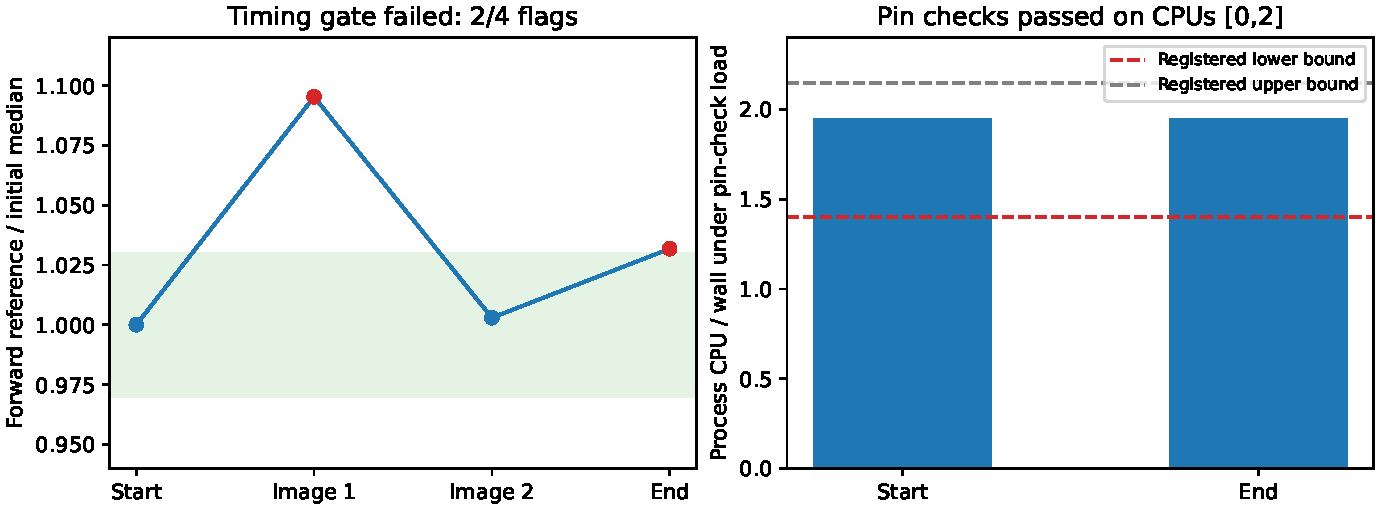
\includegraphics[width=.90\textwidth]{segmentation_extension/laptop_pcores.pdf}\caption{Two-P-core smoke: reference-timing failure alongside passing start/end pin-load checks. These are distinct gates; passing affinity verification does not override timing instability.}\label{fig:seg-laptop-pcores}\end{figure*}
